\section{Bayesian Networks and Decision Trees}
In this section we are going to define Bayesian networks and decision threes. Then we are going to compare the two decision models and choose the best model our bot can use for scouting analysis.

\subsection{Bayesian Networks}
	Bayesian networks are simple graphical models where each probability for the variable is calculated. Therefore the Bayesian networks are used for calculating new probabilities whenever new information is gathered. Bayesian networks have a  set of nodes (\ref{fig:basicbayesian}- C1,C2,C3) that are connected with directed edges. Each node in the Bayesian network must have a finite set of mutually exclusive states. By this we mean that we can only be in one state in each node. To make sure that we can calculate a result, the Bayesian network needs to be a acyclic directed graph. A node needs a conditional probability table for each of it's parents. This means that the amount of calculations in a Bayesian networks depends on the number of variables and the edges that connect them.
	
\begin{figure}[H]
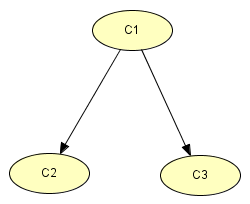
\includegraphics{Figures/BayesianPictures/BasicBayesianNetwork.png}
\caption{A simple Bayesian network}
\label{fig:basicbayesian}
\end{figure}


\subsection{Decision Trees}
Decision trees are used to represent decision problems. \ref{fig:basicdecisiontree} gives an example of a decision tree that helps investment decisions. A decision tree consists of three types of nodes: decision nodes (\ref{fig:basicdecisiontree} square boxes), chance nodes (\ref{fig:basicdecisiontree} circles) and utility nodes (\ref{fig:basicdecisiontree} triangles). The link from a decision node to a chance node is called an action, and a link from a chance node to a decision node is called a state. The idea of the decision tree is to find the path that will give us the highest utility (reward), so to make a decision tree over a decision problem, every possible path of decisions have to be shown in the tree. This will give a tree that grows exponentially with the number of decision and chance variables, so given small decision problems will require big trees, if not reduced. 
	
\begin{figure}[H]
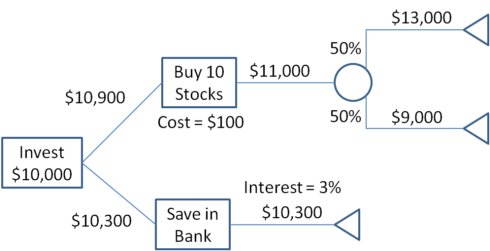
\includegraphics[scale=.8]{Figures/BayesianPictures/SimpleDecisionTree.png}
\caption{A simple decision tree \cite{sdt}}
\label{fig:basicdecisiontree}
\end{figure}

%\subsection{Conclusion}
%We decided use choose a Bayesian network solution for our problems. Since we do not know what kind of reward we would be getting for our utility function in a decision tree, It would be better to use a Bayesian network. This way we can just act on the most probable decision. Also decision networks increase in complexity way more than Bayesian networks when introducing more variables.
